

\documentclass[10pt,journal,compsoc]{IEEEtran}
% Some very useful LaTeX packages include:
% (uncomment the ones you want to load)


% *** MISC UTILITY PACKAGES ***
%
%\usepackage{ifpdf}
% Heiko Oberdiek's ifpdf.sty is very useful if you need conditional
% compilation based on whether the output is pdf or dvi.
% usage:
% \ifpdf
%   % pdf code
% \else
%   % dvi code
% \fi
% The latest version of ifpdf.sty can be obtained from:
% http://www.ctan.org/pkg/ifpdf
% Also, note that IEEEtran.cls V1.7 and later provides a builtin
% \ifCLASSINFOpdf conditional that works the same way.
% When switching from latex to pdflatex and vice-versa, the compiler may
% have to be run twice to clear warning/error messages.






% *** CITATION PACKAGES ***
%
\ifCLASSOPTIONcompsoc
  % IEEE Computer Society needs nocompress option
  % requires cite.sty v4.0 or later (November 2003)
  \usepackage[nocompress]{cite}
\else
  % normal IEEE
  \usepackage{cite}
\fi




% *** GRAPHICS RELATED PACKAGES ***
%
\ifCLASSINFOpdf
  % \usepackage[pdftex]{graphicx}
  % declare the path(s) where your graphic files are
  % \graphicspath{{../pdf/}{../jpeg/}}
  % and their extensions so you won't have to specify these with
  % every instance of \includegraphics
  % \DeclareGraphicsExtensions{.pdf,.jpeg,.png}
\else
  % or other class option (dvipsone, dvipdf, if not using dvips). graphicx
  % will default to the driver specified in the system graphics.cfg if no
  % driver is specified.
  % \usepackage[dvips]{graphicx}
  % declare the path(s) where your graphic files are
  % \graphicspath{{../eps/}}
  % and their extensions so you won't have to specify these with
  % every instance of \includegraphics
  % \DeclareGraphicsExtensions{.eps}
\fi
% graphicx was written by David Carlisle and Sebastian Rahtz. It is
% required if you want graphics, photos, etc. graphicx.sty is already
% installed on most LaTeX systems. The latest version and documentation
% can be obtained at: 
% http://www.ctan.org/pkg/graphicx
% Another good source of documentation is "Using Imported Graphics in
% LaTeX2e" by Keith Reckdahl which can be found at:
% http://www.ctan.org/pkg/epslatex
%
% latex, and pdflatex in dvi mode, support graphics in encapsulated
% postscript (.eps) format. pdflatex in pdf mode supports graphics
% in .pdf, .jpeg, .png and .mps (metapost) formats. Users should ensure
% that all non-photo figures use a vector format (.eps, .pdf, .mps) and
% not a bitmapped formats (.jpeg, .png). The IEEE frowns on bitmapped formats
% which can result in "jaggedy"/blurry rendering of lines and letters as
% well as large increases in file sizes.
%
% You can find documentation about the pdfTeX application at:
% http://www.tug.org/applications/pdftex






% *** MATH PACKAGES ***
%
%\usepackage{amsmath}
% A popular package from the American Mathematical Society that provides
% many useful and powerful commands for dealing with mathematics.
%
% Note that the amsmath package sets \interdisplaylinepenalty to 10000
% thus preventing page breaks from occurring within multiline equations. Use:
%\interdisplaylinepenalty=2500
% after loading amsmath to restore such page breaks as IEEEtran.cls normally
% does. amsmath.sty is already installed on most LaTeX systems. The latest
% version and documentation can be obtained at:
% http://www.ctan.org/pkg/amsmath





% *** SPECIALIZED LIST PACKAGES ***
%
%\usepackage{algorithmic}
% algorithmic.sty was written by Peter Williams and Rogerio Brito.
% This package provides an algorithmic environment fo describing algorithms.
% You can use the algorithmic environment in-text or within a figure
% environment to provide for a floating algorithm. Do NOT use the algorithm
% floating environment provided by algorithm.sty (by the same authors) or
% algorithm2e.sty (by Christophe Fiorio) as the IEEE does not use dedicated
% algorithm float types and packages that provide these will not provide
% correct IEEE style captions. The latest version and documentation of
% algorithmic.sty can be obtained at:
% http://www.ctan.org/pkg/algorithms
% Also of interest may be the (relatively newer and more customizable)
% algorithmicx.sty package by Szasz Janos:
% http://www.ctan.org/pkg/algorithmicx




% *** ALIGNMENT PACKAGES ***
%
%\usepackage{array}
% Frank Mittelbach's and David Carlisle's array.sty patches and improves
% the standard LaTeX2e array and tabular environments to provide better
% appearance and additional user controls. As the default LaTeX2e table
% generation code is lacking to the point of almost being broken with
% respect to the quality of the end results, all users are strongly
% advised to use an enhanced (at the very least that provided by array.sty)
% set of table tools. array.sty is already installed on most systems. The
% latest version and documentation can be obtained at:
% http://www.ctan.org/pkg/array


% IEEEtran contains the IEEEeqnarray family of commands that can be used to
% generate multiline equations as well as matrices, tables, etc., of high
% quality.




% *** SUBFIGURE PACKAGES ***
%\ifCLASSOPTIONcompsoc
%  \usepackage[caption=false,font=footnotesize,labelfont=sf,textfont=sf]{subfig}
%\else
%  \usepackage[caption=false,font=footnotesize]{subfig}
%\fi
% subfig.sty, written by Steven Douglas Cochran, is the modern replacement
% for subfigure.sty, the latter of which is no longer maintained and is
% incompatible with some LaTeX packages including fixltx2e. However,
% subfig.sty requires and automatically loads Axel Sommerfeldt's caption.sty
% which will override IEEEtran.cls' handling of captions and this will result
% in non-IEEE style figure/table captions. To prevent this problem, be sure
% and invoke subfig.sty's "caption=false" package option (available since
% subfig.sty version 1.3, 2005/06/28) as this is will preserve IEEEtran.cls
% handling of captions.
% Note that the Computer Society format requires a sans serif font rather
% than the serif font used in traditional IEEE formatting and thus the need
% to invoke different subfig.sty package options depending on whether
% compsoc mode has been enabled.
%
% The latest version and documentation of subfig.sty can be obtained at:
% http://www.ctan.org/pkg/subfig




% *** FLOAT PACKAGES ***
%
%\usepackage{fixltx2e}
% fixltx2e, the successor to the earlier fix2col.sty, was written by
% Frank Mittelbach and David Carlisle. This package corrects a few problems
% in the LaTeX2e kernel, the most notable of which is that in current
% LaTeX2e releases, the ordering of single and double column floats is not
% guaranteed to be preserved. Thus, an unpatched LaTeX2e can allow a
% single column figure to be placed prior to an earlier double column
% figure.
% Be aware that LaTeX2e kernels dated 2015 and later have fixltx2e.sty's
% corrections already built into the system in which case a warning will
% be issued if an attempt is made to load fixltx2e.sty as it is no longer
% needed.
% The latest version and documentation can be found at:
% http://www.ctan.org/pkg/fixltx2e


%\usepackage{stfloats}
% stfloats.sty was written by Sigitas Tolusis. This package gives LaTeX2e
% the ability to do double column floats at the bottom of the page as well
% as the top. (e.g., "\begin{figure*}[!b]" is not normally possible in
% LaTeX2e). It also provides a command:
%\fnbelowfloat
% to enable the placement of footnotes below bottom floats (the standard
% LaTeX2e kernel puts them above bottom floats). This is an invasive package
% which rewrites many portions of the LaTeX2e float routines. It may not work
% with other packages that modify the LaTeX2e float routines. The latest
% version and documentation can be obtained at:
% http://www.ctan.org/pkg/stfloats
% Do not use the stfloats baselinefloat ability as the IEEE does not allow
% \baselineskip to stretch. Authors submitting work to the IEEE should note
% that the IEEE rarely uses double column equations and that authors should try
% to avoid such use. Do not be tempted to use the cuted.sty or midfloat.sty
% packages (also by Sigitas Tolusis) as the IEEE does not format its papers in
% such ways.
% Do not attempt to use stfloats with fixltx2e as they are incompatible.
% Instead, use Morten Hogholm'a dblfloatfix which combines the features
% of both fixltx2e and stfloats:
%
% \usepackage{dblfloatfix}
% The latest version can be found at:
% http://www.ctan.org/pkg/dblfloatfix




%\ifCLASSOPTIONcaptionsoff
%  \usepackage[nomarkers]{endfloat}
% \let\MYoriglatexcaption\caption
% \renewcommand{\caption}[2][\relax]{\MYoriglatexcaption[#2]{#2}}
%\fi
% endfloat.sty was written by James Darrell McCauley, Jeff Goldberg and 
% Axel Sommerfeldt. This package may be useful when used in conjunction with 
% IEEEtran.cls'  captionsoff option. Some IEEE journals/societies require that
% submissions have lists of figures/tables at the end of the paper and that
% figures/tables without any captions are placed on a page by themselves at
% the end of the document. If needed, the draftcls IEEEtran class option or
% \CLASSINPUTbaselinestretch interface can be used to increase the line
% spacing as well. Be sure and use the nomarkers option of endfloat to
% prevent endfloat from "marking" where the figures would have been placed
% in the text. The two hack lines of code above are a slight modification of
% that suggested by in the endfloat docs (section 8.4.1) to ensure that
% the full captions always appear in the list of figures/tables - even if
% the user used the short optional argument of \caption[]{}.
% IEEE papers do not typically make use of \caption[]'s optional argument,
% so this should not be an issue. A similar trick can be used to disable
% captions of packages such as subfig.sty that lack options to turn off
% the subcaptions:
% For subfig.sty:
% \let\MYorigsubfloat\subfloat
% \renewcommand{\subfloat}[2][\relax]{\MYorigsubfloat[]{#2}}
% However, the above trick will not work if both optional arguments of
% the \subfloat command are used. Furthermore, there needs to be a
% description of each subfigure *somewhere* and endfloat does not add
% subfigure captions to its list of figures. Thus, the best approach is to
% avoid the use of subfigure captions (many IEEE journals avoid them anyway)
% and instead reference/explain all the subfigures within the main caption.
% The latest version of endfloat.sty and its documentation can obtained at:
% http://www.ctan.org/pkg/endfloat
%
% The IEEEtran \ifCLASSOPTIONcaptionsoff conditional can also be used
% later in the document, say, to conditionally put the References on a 
% page by themselves.




% *** PDF, URL AND HYPERLINK PACKAGES ***
%
%\usepackage{url}
% url.sty was written by Donald Arseneau. It provides better support for
% handling and breaking URLs. url.sty is already installed on most LaTeX
% systems. The latest version and documentation can be obtained at:
% http://www.ctan.org/pkg/url
% Basically, \url{my_url_here}.





% *** Do not adjust lengths that control margins, column widths, etc. ***
% *** Do not use packages that alter fonts (such as pslatex).         ***
% There should be no need to do such things with IEEEtran.cls V1.6 and later.
% (Unless specifically asked to do so by the journal or conference you plan
% to submit to, of course. )


% correct bad hyphenation here
\hyphenation{op-tical net-works semi-conduc-tor}

\usepackage[super]{nth}
\usepackage{graphicx}
\usepackage{subcaption}
\usepackage{cite}

\begin{document}
%
% paper title
% Titles are generally capitalized except for words such as a, an, and, as,
% at, but, by, for, in, nor, of, on, or, the, to and up, which are usually
% not capitalized unless they are the first or last word of the title.
% Linebreaks \\ can be used within to get better formatting as desired.
% Do not put math or special symbols in the title.
\title{Deep learning application on metagenomic data}
%
%
% author names and IEEE memberships
% note positions of commas and nonbreaking spaces ( ~ ) LaTeX will not break
% a structure at a ~ so this keeps an author's name from being broken across
% two lines.
% use \thanks{} to gain access to the first footnote area
% a separate \thanks must be used for each paragraph as LaTeX2e's \thanks
% was not built to handle multiple paragraphs
%
%
%\IEEEcompsocitemizethanks is a special \thanks that produces the bulleted
% lists the Computer Society journals use for "first footnote" author
% affiliations. Use \IEEEcompsocthanksitem which works much like \item
% for each affiliation group. When not in compsoc mode,
% \IEEEcompsocitemizethanks becomes like \thanks and
% \IEEEcompsocthanksitem becomes a line break with idention. This
% facilitates dual compilation, although admittedly the differences in the
% desired content of \author between the different types of papers makes a
% one-size-fits-all approach a daunting prospect. For instance, compsoc 
% journal papers have the author affiliations above the "Manuscript
% received ..."  text while in non-compsoc journals this is reversed. Sigh.

\author{Aly O. Abdelkareem,
        Mahmoud I. Khalil,
        Hazem M. Abbas,~\IEEEmembership{Member,~IEEE}
        and Ali H. A. Elbehery% <-this % stops a space
\IEEEcompsocitemizethanks{
\IEEEcompsocthanksitem A. O. Abdelkareem, M. I. Khalil, H. M. Abbas are with the Department
of Computer Engineering, Faculty of Engineering, Ain Shams University, Cairo, Egypt.\protect\\
% note need leading \protect in front of \\ to get a newline within \thanks as
% \\ is fragile and will error, could use \hfil\break instead.
E-mail: aly.osama@eng.asu.edu.eg
\IEEEcompsocthanksitem A. H. Elbehery was with Virlogy Institue, HelmholtzZentrum München, München, Germany.}% <-this % stops an unwanted space
\thanks{Manuscript received Dec 20, 2018; revised Jan 26, 2019.}}

% note the % following the last \IEEEmembership and also \thanks - 
% these prevent an unwanted space from occurring between the last author name
% and the end of the author line. i.e., if you had this:
% 
% \author{....lastname \thanks{...} \thanks{...} }
%                     ^------------^------------^----Do not want these spaces!
%
% a space would be appended to the last name and could cause every name on that
% line to be shifted left slightly. This is one of those "LaTeX things". For
% instance, "\textbf{A} \textbf{B}" will typeset as "A B" not "AB". To get
% "AB" then you have to do: "\textbf{A}\textbf{B}"
% \thanks is no different in this regard, so shield the last } of each \thanks
% that ends a line with a % and do not let a space in before the next \thanks.
% Spaces after \IEEEmembership other than the last one are OK (and needed) as
% you are supposed to have spaces between the names. For what it is worth,
% this is a minor point as most people would not even notice if the said evil
% space somehow managed to creep in.



% The paper headers
\markboth{IEEE/ACM Transactions on Computational Biology and Bioinformatics,~Vol.~14, No.~8, Feb~2019}%
{Abdelkareem \MakeLowercase{\textit{et al.}}: Metagenomic data analysis using deep learning}
% The only time the second header will appear is for the odd numbered pages
% after the title page when using the twoside option.
% 
% *** Note that you probably will NOT want to include the author's ***
% *** name in the headers of peer review papers.                   ***
% You can use \ifCLASSOPTIONpeerreview for conditional compilation here if
% you desire.



% The publisher's ID mark at the bottom of the page is less important with
% Computer Society journal papers as those publications place the marks
% outside of the main text columns and, therefore, unlike regular IEEE
% journals, the available text space is not reduced by their presence.
% If you want to put a publisher's ID mark on the page you can do it like
% this:
%\IEEEpubid{0000--0000/00\$00.00~\copyright~2015 IEEE}
% or like this to get the Computer Society new two part style.
%\IEEEpubid{\makebox[\columnwidth]{\hfill 0000--0000/00/\$00.00~\copyright~2015 IEEE}%
%\hspace{\columnsep}\makebox[\columnwidth]{Published by the IEEE Computer Society\hfill}}
% Remember, if you use this you must call \IEEEpubidadjcol in the second
% column for its text to clear the IEEEpubid mark (Computer Society jorunal
% papers don't need this extra clearance.)



% use for special paper notices
%\IEEEspecialpapernotice{(Invited Paper)}



% for Computer Society papers, we must declare the abstract and index terms
% PRIOR to the title within the \IEEEtitleabstractindextext IEEEtran
% command as these need to go into the title area created by \maketitle.
% As a general rule, do not put math, special symbols or citations
% in the abstract or keywords.
\IEEEtitleabstractindextext{%
\begin{abstract}
Metagenomics shows a promising understanding of function and diversity of the microbial communities due to the difficulty of studying microorganism with pure culture isolation. Moreover, the viral identification is considered one of the essential steps in studying microbial communities. Several studies show different methods to identify viruses in mixed metagenomic data and phages in host genomes, using homology and statistical techniques. These techniques have many limitations due to viral genome diversity. In this work, we propose a sequence deep neural model for viral identification of metagenomic data. For testing purpose, we generated fragments of viruses and bacteria from RefSeq genomes with different lengths to find the best hyperparameters of our model. Then, we simulated both microbiome and virome high throughput data from our test genomes dataset with aim of validating our approach. 
Finally, we applied our tool to a case study of two types of metagenomic data such as Roche 454 and Illumina.
We compared our tool to the state-of-the-art statistical and popular tool for viral identification and found the performance of VirNet much better regarding accuracy and speed on the same testing data. This tool will help us in growing our insights to natural viruses of microbial communities.

\end{abstract}

% Note that keywords are not normally used for peerreview papers.
\begin{IEEEkeywords}
	classification, deep learning, metagenomics, sequence model, virus.
\end{IEEEkeywords}}


% make the title area
\maketitle


% To allow for easy dual compilation without having to reenter the
% abstract/keywords data, the \IEEEtitleabstractindextext text will
% not be used in maketitle, but will appear (i.e., to be "transported")
% here as \IEEEdisplaynontitleabstractindextext when the compsoc 
% or transmag modes are not selected <OR> if conference mode is selected 
% - because all conference papers position the abstract like regular
% papers do.
\IEEEdisplaynontitleabstractindextext
% \IEEEdisplaynontitleabstractindextext has no effect when using
% compsoc or transmag under a non-conference mode.



% For peer review papers, you can put extra information on the cover
% page as needed:
% \ifCLASSOPTIONpeerreview
% \begin{center} \bfseries EDICS Category: 3-BBND \end{center}
% \fi
%
% For peerreview papers, this IEEEtran command inserts a page break and
% creates the second title. It will be ignored for other modes.
\IEEEpeerreviewmaketitle



\IEEEraisesectionheading{\section{Introduction}\label{sec:introduction}}
% Computer Society journal (but not conference!) papers do something unusual
% with the very first section heading (almost always called "Introduction").
% They place it ABOVE the main text! IEEEtran.cls does not automatically do
% this for you, but you can achieve this effect with the provided
% \IEEEraisesectionheading{} command. Note the need to keep any \label that
% is to refer to the section immediately after \section in the above as
% \IEEEraisesectionheading puts \section within a raised box.




% The very first letter is a 2 line initial drop letter followed
% by the rest of the first word in caps (small caps for compsoc).
% 
% form to use if the first word consists of a single letter:
% \IEEEPARstart{A}{demo} file is ....
% 
% form to use if you need the single drop letter followed by
% normal text (unknown if ever used by the IEEE):
% \IEEEPARstart{A}{}demo file is ....
% 
% Some journals put the first two words in caps:
% \IEEEPARstart{T}{his demo} file is ....
% 
% Here we have the typical use of a "T" for an initial drop letter
% and "HIS" in caps to complete the first word.
\IEEEPARstart{M}{etagenomics} is an analysis of the genetic information of the collective genomes of the microbes within a given environment based on its sampling regardless of cultivability of the cells. \cite{izard2014metagenomics}. There is a minor population of microbial organisms identified due to the difficulty in studying them using pure culture isolation. This methodology has been constrained to less than 1\% of host cells and is biased to certain species \cite{labonte2015single}.
% https://www.the-scientist.com/daily-news/most-gut-microbes-can-be-cultured-33581
Metagenomic analysis process demonstrates a promising understanding of different microorganisms. It answers some questions about the identity of microorganisms in the collection and their potential functional characterization.

Microorganisms are found everywhere on earth, and they are critical in our survival. This study, our interest is in prokaryotic microorganisms (e.g. bacteria and archaea) and viruses. Bacteria are unicellular and microscopic organisms that reproduce by binary fission. On the other hand, viruses are typically submicroscopic consists of genetic materials either DNA or RNA surrounded by a protective coat of proteins and can only replicate inside living host cells. They lack metabolic enzymes and translational machinery such as ribosomes for making proteins. There are 200 to a few thousand genes in the bacterial genomes, while the tiniest viral genomes have only three genes and the largest have up to 2000 genes.

Viruses have an impact on different microbial communities, and virus-host interaction can change many ecosystems such as human health and aquatic life. Phages or bacteriophages are viruses that infect bacteria. Furthermore, phages are abundant in different microbiome communities. The viral infection starts when virus binds to a host cell and its genome integrates with the host cell genome. The integrated viral DNA is called a provirus. It is reasonable to think that isolated viruses are just package of genes moving from one host cell to another. Scientists are using isolation and culturing techniques to study viral diversity and viral-host interactions in microbial communities. Those techniques have many limitations because there is no universal marker gene for viruses. The sequenced viruses in NCBI RefSeq database constitute approximately 5\% of known species of prokaryotic organisms \cite{roux2015viral}.

High throughput sequencing technology is used for metagenomic studies which can generate large number of read  sequences of microorganisms. The expected read length is up to 600 bp and the number of generated reads per run is up to 15 million approximately based on the sequencing platform and the library preparation methods \cite{allali2017comparison}. We can sequence mixture of prokaryotic cells and viruses in complex microbial communities in a cultivation-independent process. Sequencing of microbial samples shows contamination of viral sequences within prokaryotic population. A study found 4-17\% virus sequences in human gut prokaryotic metagenomes \cite{minot2011human}. Moreover, cellular contamination is quite frequent even with a careful purification of viral particles, and this is one of the main reasons why we need a tool that can differentiate between bacterial and viral sequences.

The broadly adopted technique to know who is in metagenomic data is to assemble the high throughput reads to contigs then search against a known genomic database using sequence alignment method in order to infer the type of microorganisms and the existence of species in a metagenomic sample. This approach is minimal because it only detects viruses almost related to those we already know. It is reported that about 15\% of viruses in the human gut microbiome and 10\% in the ocean have similarity to the known viruses \cite{ren2017virfinder}. 

Machine learning approaches have been used to classify and cluster data based on extracted features. The deep neural network is one of machine learning methods that are considered as a state of the art category for general classification problems. Deep learning shows significant improvements in several artificial intelligence tasks for example image classification, speech recognition, and natural language processing. Moreover, It shows significant results with genomic data \cite{angermueller2016deep}. %\\

In this paper, we introduce a deep sequence model, VirNet, to identify viral reads from a mixture of viral and bacterial sequences and purify viral metagenomic data from bacterial contamination as well. That will guide us to identify new viruses and potentially perform functional characterization. Additionally, it will answer many mysteries related to our understanding of their functionality and diversity in the ecosystem.


\hfill A. O. Abdelkareem

\hfill Dec 20, 2018


\section{Related Work}

There has been extensive prior work on viral identification. Recent work has focused on identifying phages in bacterial genomes. Several methods have used similarity search by sequence alignment with the reference genomes in order to find viral contigs. Most of the recent tools fall under three categories based on the sample structure such as:
\begin{enumerate}
	\item phages from prokaryotic genomes
	\item viral sequences in mixed metagenomic datasets
	\item phages and viral sequences. 
\end{enumerate} 

There are many software packages to find phages from prokaryotic genomes such as Phage\_Finder \cite{fouts2006phage_finder}, Prophinder \cite{lima2008prophinder}, PHAST\cite{zhou2011phast}, and PhiSpy \cite{akhter2012phispy}. These tools are using similarity search to known virus databases using features such as genes. Some of them such as PhiSpy integrates other features such as  unique virus k-mers, AT and GC skew, protein length and transcription strand direction. They have many limitations as they failed to detect viral sequences in metagenomic data as the databases are outdated, limited and don't represent viral diversity in the environment. Moreover, It is not optimized to process a large number of contigs \cite{roux2015virsorter} as they depend on alignment and homology processing limitations. 

The second category is able to detect viral sequences in mixed metagenomic datasets such as VIROME \cite{wommack2012virome} and MetaVir\cite{roux2011metavir}. They are using similarity search with the databases same as the first category. Additionally, they are searching against proteins. There are more packages such as DIAMOND \cite{buchfink2014Diamond} or Centrifuge \cite{kim2016centrifuge} which are much faster and efficient than the former tools for microbial classification. Again, The limitation of this approach is using limited known reference databases. 

The third category of software packages such as VirSorter \cite{roux2015virsorter} is able to detect phages and viral sequences. VirSorter is using similarity search to viral databases and integrates other features related to analysis of sequence genes such as enrichment of viral-like genes, enrichment of uncharacterized genes and viral hallmark gene. These features make the identification more accurate but it still suffer limitations. One of the limitations is the requirements of having at least 3 genes within the contig because the smallest virus genome contains 3 genes because the smallest virus discovered has 3 genes only so it has the same limitations as previous techniques because of using homology strategy. Moreover, it cannot work with short fragments or contigs and it is very slow in processing metagenomic datasets. 

Recently VirFinder \cite{ren2017virfinder} applied machine learning techniques. VirFinder is a statistical method based on the logistic regression model. It uses the K-mer feature which is considered as a discrimination feature for different sequence problems. It shows a great success with short sequences too and They found a great k-mer similarity score with viruses within other prokaryotic genomes. 

% need to write deep learning techniques in fragments classification

In this paper, we are using deep learning techniques which is much more suitable to sequence problems and also shows significant improvements to other current machine learning models. In deep neural networks, the model will extract the most appropriate features during training which lead to better identification accuracy and sensitivity. 

\section{Materials and Methods}

\subsection{Building training and testing dataset}
We downloaded viruses, bacteria and archaea genomes from RefSeq database then we divided them randomly into a train and test genomes with 80\% of total base pairs in training. Table \ref{table:genome_stats} shows the number of genomes we used in training and testing. We processed all available viral genomes until Nov. \nth{1}, 2017 and a sample from prokaryotic genomes due to the huge number of available prokaryotic genomes. Then, we converted the viral genomes into non-overlapping fragments of different lengths n = \{100, 500, 1000, 3000\}. We generated an approximate number of non-overlapping fragments of prokaryotic genomes with the same lengths randomly as well. (Table \ref{table:fragments_stats}). We balanced the data of both classes using random under-sampling technique to avoid the bias to the majority class with the deep neural network. Figure \ref{fig:data_pipline} shows more details for data pipeline.

\begin{figure}[!htbp]
	\centering
	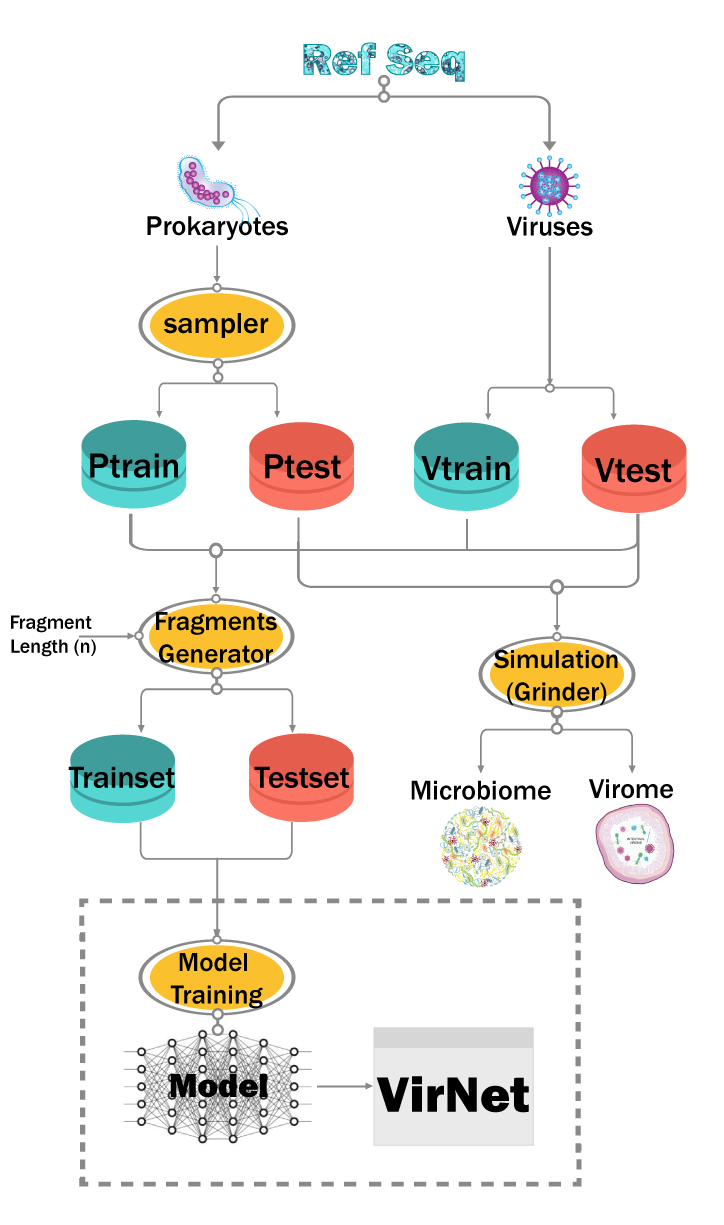
\includegraphics[width=\columnwidth]{imgs/data_pipeline.PNG}
	\caption{VirNet Data Pipeline}
	\label{fig:data_pipline}
\end{figure}

\begin{table}[!htbp]
	\centering
	\begin{tabular}{||c c c c||} 
		Genome & Train & Test & Total \\ [0.5ex] 
		\hline\hline
		Viruses & 7686  & 1870 & 9556 \\ 
		Prokaryotes & 143241  & 35543 & 178784  \\ [1ex] 
	\end{tabular}
	\caption{The number of used genomes from RefSeq}
	\label{table:genome_stats}
\end{table}

\begin{table}[h!]
	\centering
	\begin{tabular}{||c c c||} 
		Fragment Length (N) & Train & Test \\ [0.5ex] 
		\hline\hline
		100 bp & 2088863  & 527020  \\ 
		500 bp & 420857  & 106168  \\
		1000 bp & 212253  & 53528  \\
		3000 bp & 73163  & 18425  \\ [1ex] 
	\end{tabular}
	\caption{The number of fragments generated from viruses genomes}
	\label{table:fragments_stats}
\end{table}

\subsection{Generating simulated virome and microbiome}
Grinder \cite{angly2012grinder} is an open-source tool commonly used for generating a simulate amplicon and shotgun metagenomic datasets from reference genomes. 
We generated two metagenomic data of virome and microbiome of 1M reads and fragment length 100bp using Grinder with our reference test genomes to simulate shotgun metagenomic sequences in order to verify the ability of our tool to detect viral reads in metagenomic data instead of generated fragments from the reference genomes. The virome data has 75\% of viral reads while microbiome has 25\%. Moreover, we used Illumina error model indicated by mutation\_dist poly4 3e-3 3.3e-8 and mutation ratio 91:9 (9 indels for each 91 substitution mutations) because for Illumina indel errors occur more often than substitution errors \cite{laehnemann2015denoising}. Table \ref{table:simulate_stats} shows simulated data statistics.  \\

\begin{table}[!htbp]
	\centering
	\begin{tabular}{||c c c||} 
		& Microbiome & Virome \\ [0.5ex] 
		\hline\hline
		Bacteria Length & 75450367  bp  & 17551396 bp  \\
		Bacteria Genomes & 1488 & 422\\
		Bacterial reads & 803742 & 176059\\
		Viruses Length & 25133078 bp  & 52609236 bp  \\ 
		Viruses Genomes & 845 & 1870\\
		Viral reads & 196258 & 823941 \\  
		Viral Ratio & 25.00\% & 75.00\% \\ 
		Library coverage &  0.994x &  1.001x  \\
		Diversity (richness) & 2302 & 2726 \\ [1ex]
	\end{tabular}
	\caption{Grinder Simulated Metagenome}
	\label{table:simulate_stats}
\end{table}


\subsection{Case Study: Real metagenomic data}
We applied our tool to two real metagenomes as a case study
\begin{enumerate}
	\item \textbf{454}: Subtropical freshwater microbial and viral metagenome (SRR648314).\
	\item \textbf{Illumina}: Lake Michigan virome (SRX995836).
\end{enumerate}
Our tool is able to read not only fasta files and fastq files. Furthermore, it is able to deal with paired-end reads i.e. if one of the two pairs is identified as a virus, the other should be the same. If there are conflicts between the classifications of the two pairs; this pair could be denoted as ambiguous.

\subsection{Deep Learning Model}
Recurrent neural networks (RNN), long short-term memory (LSTM) \cite{hochreiter1997long} and gated recurrent neural networks (GRU) \cite{chung2014empirical} can model complex sequences and have been used for sequence modeling problems.

Our deep learning model is implemented as an attentional encoder network (Figure \ref{fig:encoder}). An input sequence  $\mathbf{x = (x_{1} , \ldots{} , x_{m} )}$  and calculates a forward sequence of hidden states  ($\mathbf{\overrightarrow{h_{1}}}$,\ldots{},$\mathbf{ \overrightarrow{h_{m}}}$). The hidden states $\mathbf{\overrightarrow{h_{j}}}$  are averaged to obtain the attention vector $\mathbf{h_{j}}$ representing the context vector from the input sequence.

Embedding layer maps discrete input words to dense vectors for computational efficiency before feeding this sequence to LSTM/GRU Layers. The attentional network could learn how to extract suitable features from the raw data and can attend to previous DNA nucleotide within the same input sequence. 

LSTM encoder have 3 gates to protect and control the cell state, the input gate denoted $\mathbf{i}$ which defines how much of the newly computed state you want to let through, forget gate denoted $\mathbf{f}$ that decides what information is to be kept and what is to be thrown away,  the output of the update gate denoted $\mathbf{U}$ that's used to update the cell state and the output of the LSTM cell $\mathbf{o}$ .$\mathbf{W}$ is the recurrent connection at the previous hidden layer and current hidden layer and $\mathbf{C}$ is the internal memory of the unit  as shown in the following equations \newline
$\mathbf{i_{t}=\sigma(x_{t}U^i + h_{t-1}W^i)}$ \newline
$\mathbf{f_{t}=\sigma(x_{t}U^f + h_{t-1}W^f)}$ \newline
$\mathbf{o_{t}=\sigma(x_{t}U^o + h_{t-1}W^o)}$. 

GRU encoder is same as LSTM except it has only 2 gates, Reset gate denoted $\mathbf{r}$ that determines how to combine the new input with the previously saved input state and the update gate denoted $\mathbf{z}$ that defines the amount of information to keep around, as defined  in the following equations \newline
$\mathbf{z_{t}=\sigma(x_{t}U^z + h_{t-1}W^z)}$ \newline
$\mathbf{r_{t}=\sigma(x_{t}U^r + h_{t-1}W^r)}$ \newline
$\mathbf{\overline{h_{t}} = tanh(x_{t}U^h + (r_{t} * h_{t-1})W^h )}$ \newline
$\mathbf{ h_{t} = (1-z_{t})h_{t-1} +z_{t}\overline{h_{t}}}$.


The attentional neural model was trained with the DNA nucleotide bases with fragments with different lengths. The model will predict in a binary output format whether this fragment is viral or non-viral.

The top-performing model (Figure \ref{fig:model_diagram}) consists of an input embedding layer of size 128 mapping input DNA nucleotide tokens into an embedding space, that is fed to an LSTM layer. The forward sequence $\mathbf{\overrightarrow{h_{j}}}$ is then averaged together to create an attentional vector representing token context within the same fragment. A dropout layer was added after the attentional layer to avoid overfitting over the input data.

LSTM layer was performing better as in \ref{table:hyper_results} than the GRU cell. GRU encoder having less gates than LSTM model make it faster and easier to converge, but depedending on the size and the format of the input data. LSTM with more gates would be slower but will outperform GRU encoder type.

The input sequence is divided into 5 grams sized tokens these tokens are then treated as a single word (Figure \ref{fig:encoder}). This single token is mapped as a point in the embedding space created during training the neural model.

During training, all parameters are optimized jointly using Adam to maximize the conditional probability of tokens found together to predict if an input sequence is viral or not.

In this model, an early stopping mechanism was used as a form of regularization to avoid over-fitting over the data while making more epochs over the data. The early stopping mechanism was used with patience of 3 non -improving consecutive epochs; the neural model will stop training while saving the latest improving checkpoint over the validation set defined.

\subsection{Hyperparameters optimization}

Model parameters affect the performance of the deep learning model, and they control the behavior of the training algorithm as well. We selected the grid search technique in order to find the most suitable parameters. The grid search is considered a traditional technique for hyperparameters optimization and it brute force different combinations. We ran several experiments on 20\% of our training set for 500 bp. Then, we divided it into training, validation, and testing set with the following percentages 70\%, 10\%, and 20\%. These experiments were designed to find the best parameters for the number of recurrent layers, the embedding size for each layer and the input sub-words (ngram). Our reported results (Table \ref{table:hyper_results}) show that the best parameters setup is for 2 layers, 128 embedding size, and 5 ngram. 

We ran other experiments with the same parameters to check the ability of our model with other configuration, so we changed different parameters separately such as embedding size to 256 neurons, the number of layers to 3 and the recurrent cell type to GRU instead of LSTM. We found a slightly less accuracy and ROC-AUC scores but the training time was much more than the best parameters configuration as expected due to increasing number of neural network parameters.

\begin{table}[!htbp]
	\centering
	\begin{tabular}{||c c c c c||} 
		\#Layers & Embedding & Ngram & ROC-AUC & Accuracy \\ [0.5ex] 
		\hline\hline
		1      & 32                      & 3     & 0.8     & 73.66    \\
		1      & 32                      & 5     & 0.83    & 76.42    \\
		1      & 32                      & 7     & 0.79    & 72.11    \\
		1      & 64                      & 3     & 0.83    & 76.1     \\
		1      & 64                      & 5     & 0.83    & 75.98    \\
		1      & 64                      & 7     & 0.77    & 69.96    \\
		1      & 128                     & 3     & 0.83    & 75.76    \\
		1      & 128                     & 5     & 0.85    & 77.41    \\
		1      & 128                     & 7     & 0.78    & 70.93    \\
		2      & 32                      & 3     & 0.8     & 73.25    \\
		2      & 32                      & 5     & 0.83    & 76.49    \\
		2      & 32                      & 7     & 0.79    & 72.82    \\
		2      & 64                      & 3     & 0.81    & 73.96    \\
		2      & 64                      & 5     & 0.84    & 76.46    \\
		2      & 64                      & 7     & 0.78    & 72.53    \\
		2      & 128                     & 3     & 0.83    & 76.15    \\
		\textbf{2} & \textbf{128}            & \textbf{5} & \textbf{0.85} & \textbf{77.9} \\
		2      & 128                     & 7     & 0.78    & 70.63    \\[1ex]
	\end{tabular}
	\caption{Hyperparamters optimization results}
	\label{table:hyper_results}
\end{table}


\begin{figure}[!htbp]
	\centering
	\begin{subfigure}{0.4\textwidth}
		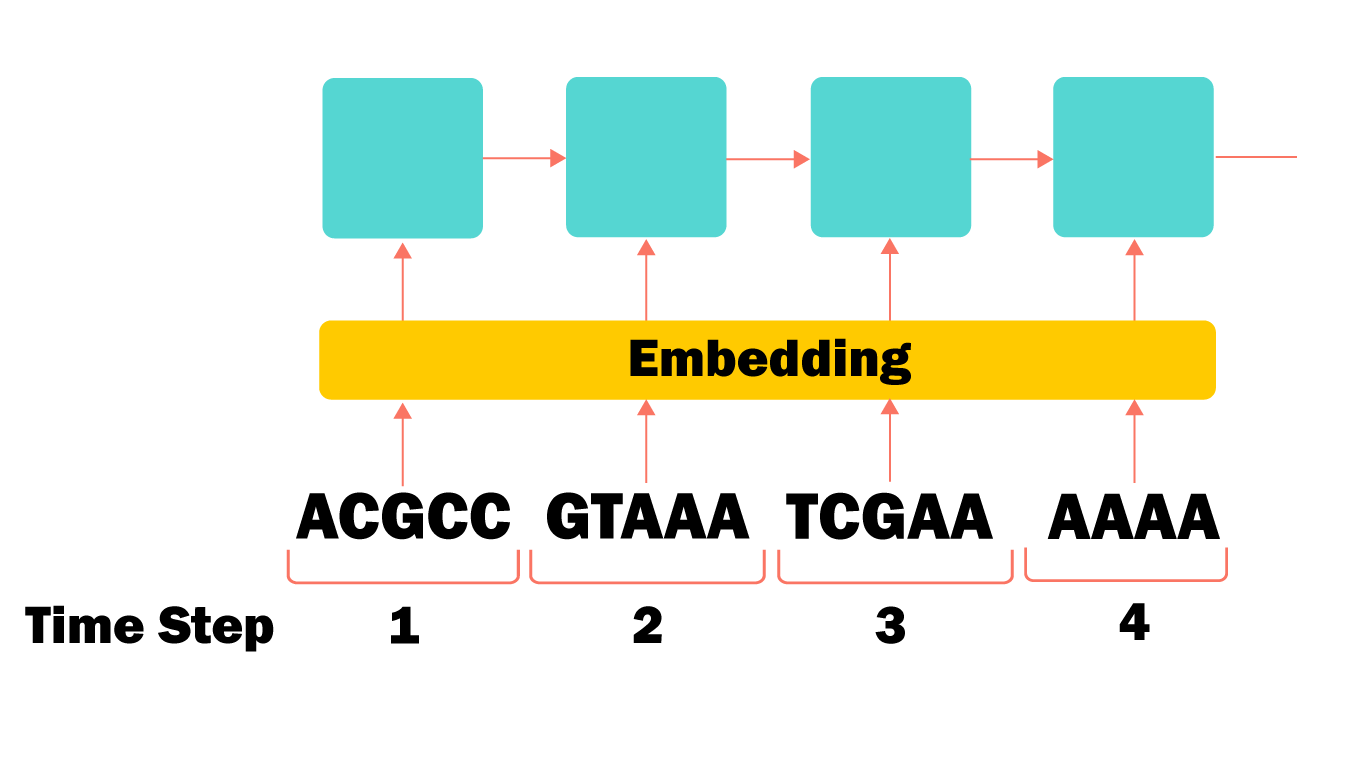
\includegraphics[width=\linewidth]{imgs/encoder.PNG}
		\caption{Embedding Layer} 
		\label{fig:encoder}
	\end{subfigure}
	\hspace*{\fill} % separation between the subfigures
	\begin{subfigure}{0.4\textwidth}
		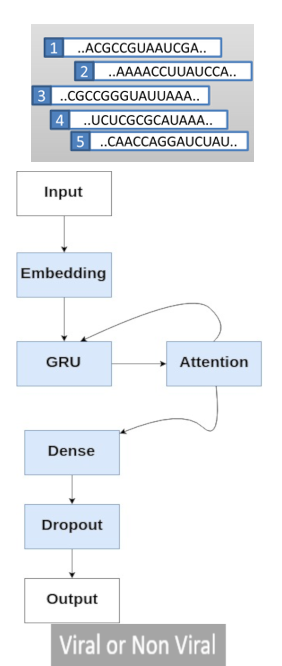
\includegraphics[width=\linewidth]{imgs/model_diagram.PNG}
		\caption{Neural network model architecture} 
		\label{fig:model_diagram}
	\end{subfigure}
	\caption{VirNet model} 
	\label{fig:model_arch}
\end{figure}

\section{Results}

\subsection{Results for generated fragments}
We tested VirNet on different lengths of fragments n= \{100, 500, 1000, 3000\} from our testing set of viruses and prokaryotes RefSeq genomes. Moreover, we compared the output results to VirFinder results on the same training and testing data. VirNet predictions outperformed VirFinder for fragments with length 500, 1000 and 3000 (Figure \ref{fig:accuracy_graph}). The model reached to 82.82\% of accuracy whereas VirFinder tool obtained 75.61\%. Moreover, VirFinder can perdict the short fragments with length 100. Figures \ref{fig:roc_auc_virfindera} and \ref{fig:roc_auc_virneta} shows ROC-AUC curves of both tools on the testing set. Table \ref{table:virfinder_results} shows the comparison between both tools in terms of accuracy, average precision and average recall.

%\begin{table}[h!]
%	\centering
%	\begin{tabular}{||c l l l l l l l l||} 
%		Length(N) &	\multicolumn{2}{l}{Accuracy} & \multicolumn{2}{l}{Avg. Precision} & \multicolumn{2}{l}{Avg. Recall} &	\multicolumn{2}{l}{ROC-AUC} \\ [0.5ex] 
%		& VirNet & VirFinder & VirNet & VirFinder & VirNet & VirFinder & VirNet & VirFinder \\
%				\hline\hline
%		100 & 71.29\% &	63.9\%	& 0.72 & 0.64 & 0.71 & 0.64 & 0.80 & 0.64 \\
%		500 & 82.82\% &	75.61\% & 0.83 &	0.76 & 0.83 & 0.76 & 0.9 & 0.75 \\
%		1000 & 86.82\% &	80.28\% &  0.87 & 0.82 & 0.87 & 0.80 & 0.93 & 0.78 \\
%		3000 & 90.10\% &	87.11\% & 0.91 & 0.88 & 0.90 & 0.87 & 0.94 & 0.83\\[1ex]
%	\end{tabular}
%	\caption{VirFinder Results on our test-set}
%	\label{table:virfinder_results}
%\end{table}

\begin{table}[!htbp]
	\centering
	\begin{tabular}{||c l l l l l l||} 
		Length(N) &	\multicolumn{2}{l}{Accuracy} & \multicolumn{2}{l}{Avg. Precision} & \multicolumn{2}{l}{Avg. Recall}\\ [0.5ex] 
		& VirNet & VirFinder & VirNet & VirFinder & VirNet & VirFinder \\
		\hline\hline
		100 & 71.29\% &	63.9\%	& 0.72 & 0.64 & 0.71 & 0.64 \\
		500 & 82.82\% &	75.61\% & 0.83 &	0.76 & 0.83 & 0.76\\
		1000 & 86.82\% &	80.28\% &  0.87 & 0.82 & 0.87 & 0.80 \\
		3000 & 90.10\% &	87.11\% & 0.91 & 0.88 & 0.90 & 0.87 \\[1ex]
	\end{tabular}
	\caption{Comparison on fragments test-set}
	\label{table:virfinder_results}
\end{table}

\subsection{Results for simulated metagenomes}

As mentioned before, we tested VirNet on a simulated metagenomes of 100 bp and we found that VirNet performed much better than VirFinder. VirNet shows accuracy is 71.3\% on the virome data and 72.14\% on the microbiome data while VirFinder is 62.77\% on the virome data and 64.49\% on the microbiome data Table \ref{table:virfinder_results_simulated}). The ROC-AUC curves of both tools shows the difference between them (Figures \ref{fig:roc_auc_virfinderb} and \ref{fig:roc_auc_virnetb}).

\begin{figure}
	\centering
	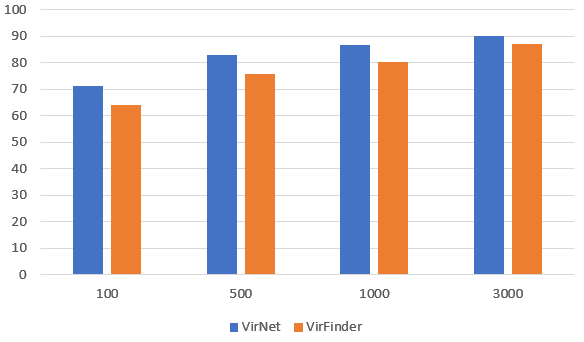
\includegraphics[width=\columnwidth]{imgs/accuracy_graph.PNG}
	\caption{VirNet vs VirFinder Accuracy}
	\label{fig:accuracy_graph}
\end{figure}


\begin{figure}[!htbp]
	\centering
	\begin{subfigure}{0.3\textwidth}
		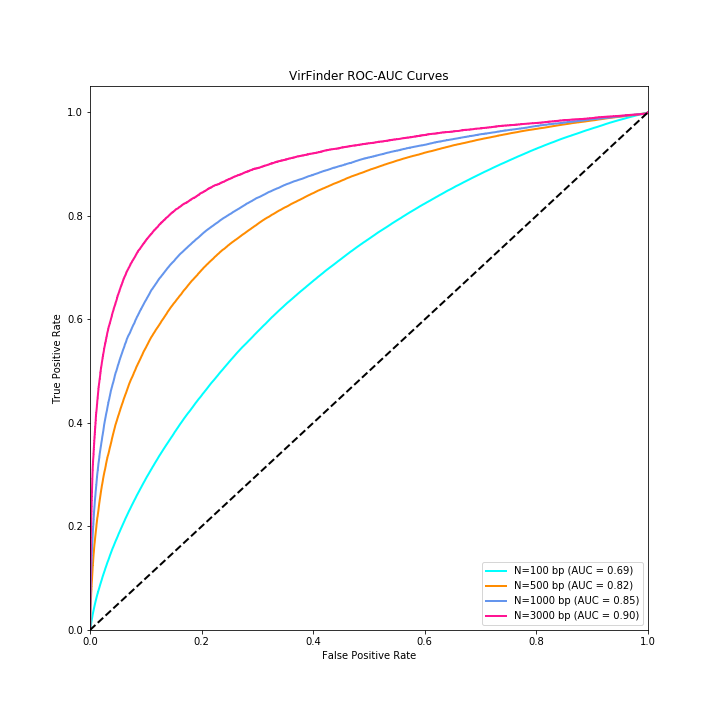
\includegraphics[width=\linewidth]{imgs/roc_auc.png}
		\caption{VirFinder with generated fragments} 
		\label{fig:roc_auc_virfindera}
	\end{subfigure}
	\begin{subfigure}{0.3\textwidth}
		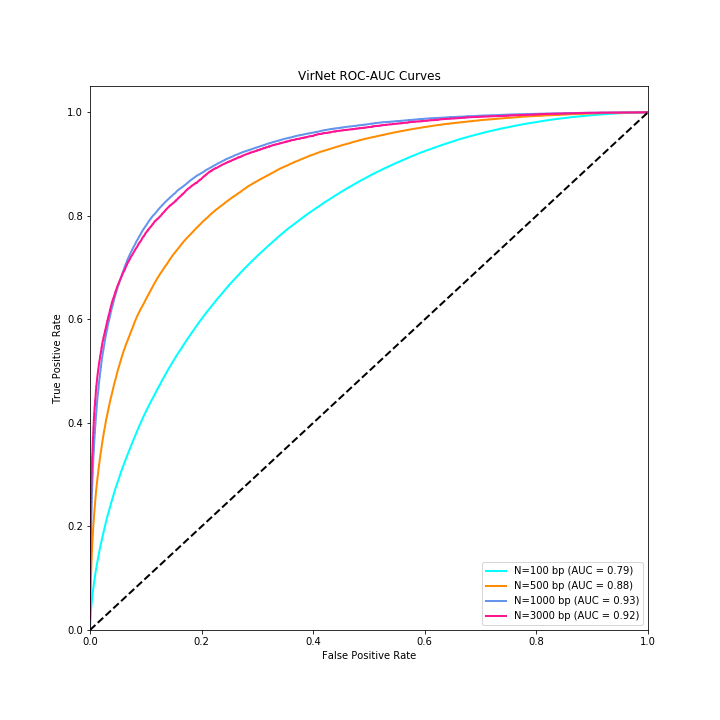
\includegraphics[width=\linewidth]{imgs/virnet_roc_auc.png}
		\caption{VirNet with generated fragments} 
		\label{fig:roc_auc_virneta}
	\end{subfigure}
	\begin{subfigure}{0.3\textwidth}
		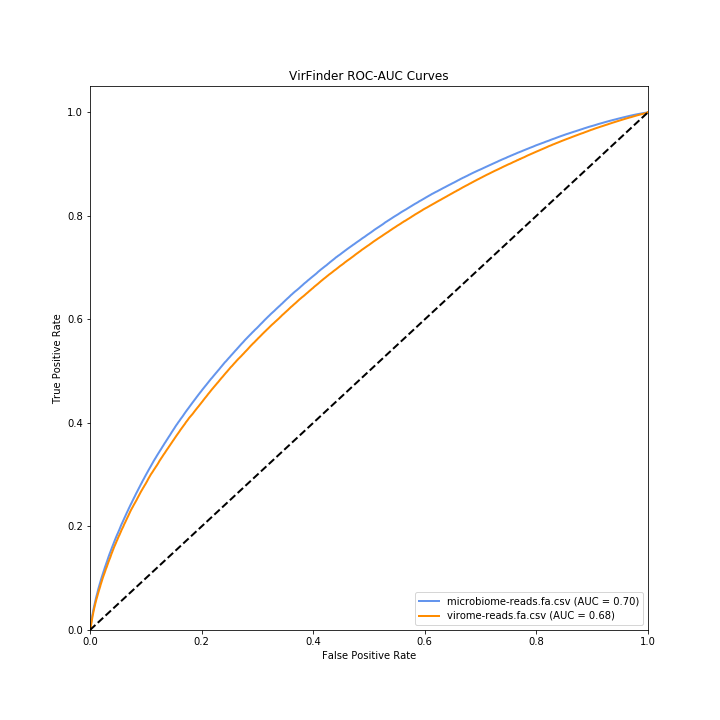
\includegraphics[width=\linewidth]{imgs/roc_auc_simulated.png}
		\caption{VirFinder with simulated genomes} 
		\label{fig:roc_auc_virfinderb}
	\end{subfigure}
	\begin{subfigure}{0.3\textwidth}
		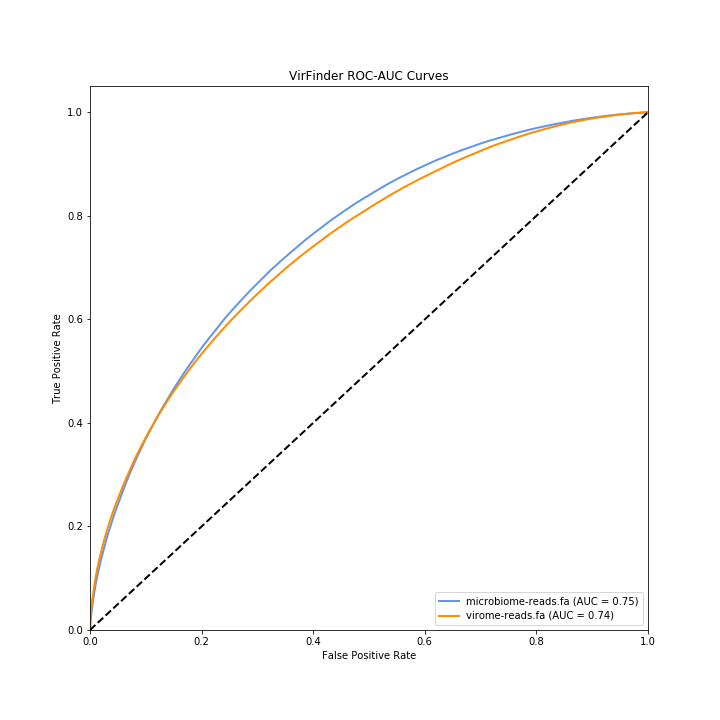
\includegraphics[width=\linewidth]{imgs/virnet_roc_auc_simulated.png}
		\caption{VirNet with simulated genomes} 
		\label{fig:roc_auc_virnetb}
	\end{subfigure}
	\caption{ROC-AUC curves on fragments and simulated metagenomes} 
	\label{fig:roc_auc_virfinder}
\end{figure}



\begin{table}[!htbp]
	\centering
	\begin{tabular}{||l l l l l l l||} 
		Metagenome &	\multicolumn{2}{l}{Accuracy} & \multicolumn{2}{l}{Avg. Precision} & \multicolumn{2}{l}{Avg. Recall}\\ [0.5ex] 
		& VirNet & VirFinder & VirNet & VirFinder & VirNet & VirFinder \\
		\hline\hline
		Virome & 71.3\% &	62.77\%	& 0.71 & 0.63 & 0.72 & 0.62 \\
		Microbiome &	72.14\% & 64.49\% &	0.73 & 0.65 & 0.73 & 0.64 \\ [1ex]
	\end{tabular}
	\caption{Simulated Metagenomes Results}
	\label{table:virfinder_results_simulated}
\end{table}

\subsection{Results for real data}
we applied the tool on two real data with accession numbers SRR648314, SRX995836\_1 and SRX995836\_2. Table \ref{table:virnet_results_real} shows that our tool could able work on the real metagenomic data. 

\begin{table}[]
	\centering
	\begin{tabular}{||llll||}
		& SRR648314 & SRR1974517/1 & SRR1974517/2 \\
		\hline\hline
		Viral     & 39447     & 579697       & 590869       \\
		Non Viral & 20866     & 1055975      & 1044803      \\
		Total     & 60313     & 1635672      & 1635672     
	\end{tabular}
	\caption{VirNet results on real data}
	\label{table:virnet_results_real}
\end{table}

\subsection{VirNet processing speed}
Using GPUs is an advantage for our tool and make it very fast and scalable in processing massive amount of metagenomic reads simultaneously. The training process is around 5 hours with 2 million reads, while the prediction process is around 30 seconds on 1 million reads using Nvidia GeForce GTX 1080 Ti. On the other hand, VirFinder processing the reads on a single CPU less than VirNet by around 82 times. We can avoid that by using parallel CPU threads for VirFinder but in case you want to retrain it with new data, it will take a couple of days.

\section{Discussion}

In our tool, there are no handmade features as the network will learn how to extract appropriate features of the raw data. It shows better accuracy as it is trained with the updated viral databases with a good statistical model. This helps us to generalize this model with all genomes and to make a generalized model for sequence classification. We are also able to identify the short viral sequences as LSTM learns from the dependences between the input sequence. 

There is no evidence that these training prokaryotic genomes don't have a viral infection or not. Cleaning the training genomes might give us better accuracy but based on sampling and randomizing prokaryotic fragments, our training data may not contain proviruses. 

For the trained deep learning model, using a sliding window over the input DNA sequence might improve our model, the only drawback of this technique is the slow training and inference time of input sequences, Also using an adaptive learning rate decaying over time steps during the training might improve the model performance, but will need more tuning over the input data.

\section{Conclusion}

This attentional neural deep learning network was able to achieve state of the art results on viral identification from high throughput sequences. Our approach is able to classify short fragments as well. Experimental results validate our approach for identification with an accuracy of more than 83\%. According to these results, Our model would help us in understanding viruses in various microbial communities and discovering new species of viruses.



% An example of a floating figure using the graphicx package.
% Note that \label must occur AFTER (or within) \caption.
% For figures, \caption should occur after the \includegraphics.
% Note that IEEEtran v1.7 and later has special internal code that
% is designed to preserve the operation of \label within \caption
% even when the captionsoff option is in effect. However, because
% of issues like this, it may be the safest practice to put all your
% \label just after \caption rather than within \caption{}.
%
% Reminder: the "draftcls" or "draftclsnofoot", not "draft", class
% option should be used if it is desired that the figures are to be
% displayed while in draft mode.
%
%\begin{figure}[!t]
%\centering
%\includegraphics[width=2.5in]{myfigure}
% where an .eps filename suffix will be assumed under latex, 
% and a .pdf suffix will be assumed for pdflatex; or what has been declared
% via \DeclareGraphicsExtensions.
%\caption{Simulation results for the network.}
%\label{fig_sim}
%\end{figure}

% Note that the IEEE typically puts floats only at the top, even when this
% results in a large percentage of a column being occupied by floats.
% However, the Computer Society has been known to put floats at the bottom.


% An example of a double column floating figure using two subfigures.
% (The subfig.sty package must be loaded for this to work.)
% The subfigure \label commands are set within each subfloat command,
% and the \label for the overall figure must come after \caption.
% \hfil is used as a separator to get equal spacing.
% Watch out that the combined width of all the subfigures on a 
% line do not exceed the text width or a line break will occur.
%
%\begin{figure*}[!t]
%\centering
%\subfloat[Case I]{\includegraphics[width=2.5in]{box}%
%\label{fig_first_case}}
%\hfil
%\subfloat[Case II]{\includegraphics[width=2.5in]{box}%
%\label{fig_second_case}}
%\caption{Simulation results for the network.}
%\label{fig_sim}
%\end{figure*}
%
% Note that often IEEE papers with subfigures do not employ subfigure
% captions (using the optional argument to \subfloat[]), but instead will
% reference/describe all of them (a), (b), etc., within the main caption.
% Be aware that for subfig.sty to generate the (a), (b), etc., subfigure
% labels, the optional argument to \subfloat must be present. If a
% subcaption is not desired, just leave its contents blank,
% e.g., \subfloat[].


% An example of a floating table. Note that, for IEEE style tables, the
% \caption command should come BEFORE the table and, given that table
% captions serve much like titles, are usually capitalized except for words
% such as a, an, and, as, at, but, by, for, in, nor, of, on, or, the, to
% and up, which are usually not capitalized unless they are the first or
% last word of the caption. Table text will default to \footnotesize as
% the IEEE normally uses this smaller font for tables.
% The \label must come after \caption as always.
%
%\begin{table}[!t]
%% increase table row spacing, adjust to taste
%\renewcommand{\arraystretch}{1.3}
% if using array.sty, it might be a good idea to tweak the value of
% \extrarowheight as needed to properly center the text within the cells
%\caption{An Example of a Table}
%\label{table_example}
%\centering
%% Some packages, such as MDW tools, offer better commands for making tables
%% than the plain LaTeX2e tabular which is used here.
%\begin{tabular}{|c||c|}
%\hline
%One & Two\\
%\hline
%Three & Four\\
%\hline
%\end{tabular}
%\end{table}


% Note that the IEEE does not put floats in the very first column
% - or typically anywhere on the first page for that matter. Also,
% in-text middle ("here") positioning is typically not used, but it
% is allowed and encouraged for Computer Society conferences (but
% not Computer Society journals). Most IEEE journals/conferences use
% top floats exclusively. 
% Note that, LaTeX2e, unlike IEEE journals/conferences, places
% footnotes above bottom floats. This can be corrected via the
% \fnbelowfloat command of the stfloats package.



% if have a single appendix:
%\appendix[Proof of the Zonklar Equations]
% or
%\appendix  % for no appendix heading
% do not use \section anymore after \appendix, only \section*
% is possibly needed

% use appendices with more than one appendix
% then use \section to start each appendix
% you must declare a \section before using any
% \subsection or using \label (\appendices by itself
% starts a section numbered zero.)
%


\appendices
\section{Proof of the Attention models}
Appendix one text goes here.

% you can choose not to have a title for an appendix
% if you want by leaving the argument blank
\section{}
Appendix two text goes here.




\section*{Availability of data}

VirNet is an open-source python package at https://github.com/alyosama/virnet. RefSeq genomes used are publicly available online via NCBI. All other generated data used in this study are available from the corresponding author on a request. 

% use section* for acknowledgment
\ifCLASSOPTIONcompsoc
  % The Computer Society usually uses the plural form
  \section*{Acknowledgments}
\else
  % regular IEEE prefers the singular form
  \section*{Acknowledgment}
\fi

We acknowledge Eng. Mayada Elsayed for designing the figures.


% Can use something like this to put references on a page
% by themselves when using endfloat and the captionsoff option.
\ifCLASSOPTIONcaptionsoff
  \newpage
\fi



% trigger a \newpage just before the given reference
% number - used to balance the columns on the last page
% adjust value as needed - may need to be readjusted if
% the document is modified later
%\IEEEtriggeratref{8}
% The "triggered" command can be changed if desired:
%\IEEEtriggercmd{\enlargethispage{-5in}}

% references section

% can use a bibliography generated by BibTeX as a .bbl file
% BibTeX documentation can be easily obtained at:
% http://mirror.ctan.org/biblio/bibtex/contrib/doc/
% The IEEEtran BibTeX style support page is at:
% http://www.michaelshell.org/tex/ieeetran/bibtex/
%\bibliographystyle{IEEEtran}
% argument is your BibTeX string definitions and bibliography database(s)
%\bibliography{IEEEabrv,../bib/paper}
%
% <OR> manually copy in the resultant .bbl file
% set second argument of \begin to the number of references
% (used to reserve space for the reference number labels box)
%\begin{thebibliography}{1}

%\bibitem{IEEEhowto:kopka}
%H.~Kopka and P.~W. Daly, \emph{A Guide to \LaTeX}, 3rd~ed.\hskip 1em plus
% 0.5em minus 0.4em\relax Harlow, England: Addison-Wesley, 1999.

%\end{thebibliography}

\bibliography{scholar}
\bibliographystyle{plain}



% biography section
% 
% If you have an EPS/PDF photo (graphicx package needed) extra braces are
% needed around the contents of the optional argument to biography to prevent
% the LaTeX parser from getting confused when it sees the complicated
% \includegraphics command within an optional argument. (You could create
% your own custom macro containing the \includegraphics command to make things
% simpler here.)
%\begin{IEEEbiography}[{\includegraphics[width=1in,height=1.25in,clip,keepaspectratio]{mshell}}]{Michael Shell}
% or if you just want to reserve a space for a photo:

\begin{IEEEbiography}{Aly O. Abdelkareem}
Biography text here.
\end{IEEEbiography}

% if you will not have a photo at all:
\begin{IEEEbiographynophoto}{Mahmoud I. Khalil}
Biography text here.
\end{IEEEbiographynophoto}

% insert where needed to balance the two columns on the last page with
% biographies
%\newpage

\begin{IEEEbiographynophoto}{Hazem M. Abbas}
Biography text here.
\end{IEEEbiographynophoto}


\begin{IEEEbiographynophoto}{Ali H. Elbehery}
	Biography text here.
\end{IEEEbiographynophoto}

% You can push biographies down or up by placing
% a \vfill before or after them. The appropriate
% use of \vfill depends on what kind of text is
% on the last page and whether or not the columns
% are being equalized.

%\vfill

% Can be used to pull up biographies so that the bottom of the last one
% is flush with the other column.
%\enlargethispage{-5in}



% that's all folks
\end{document}


